\chapter{Projekt}
Příloha slouží pro splnění části požadavků projektu ze předmětu Elektronické publikování.

\textbf{Zvýrazněný text}.

\begin{comment}
  \section{Zakomentovaná sekce}
  Obsah zakomentované sekce
\end{comment}

Graf výkonnosti pracovníka během 8hodinového pracovního dne:

\begin{gnuplot}[terminal=pdf,terminaloptions=color]
    unset key
    set samples 10000
    set format '%g'
    set xlabel "Počet odpracovaných hodin"
    set ylabel "Výkonnost"
    set xrange [0:8]
    set yrange [0:1]
    plot sin((x/3.35)+0.75)
\end{gnuplot}

\begin{figure}
  \begin{center}
  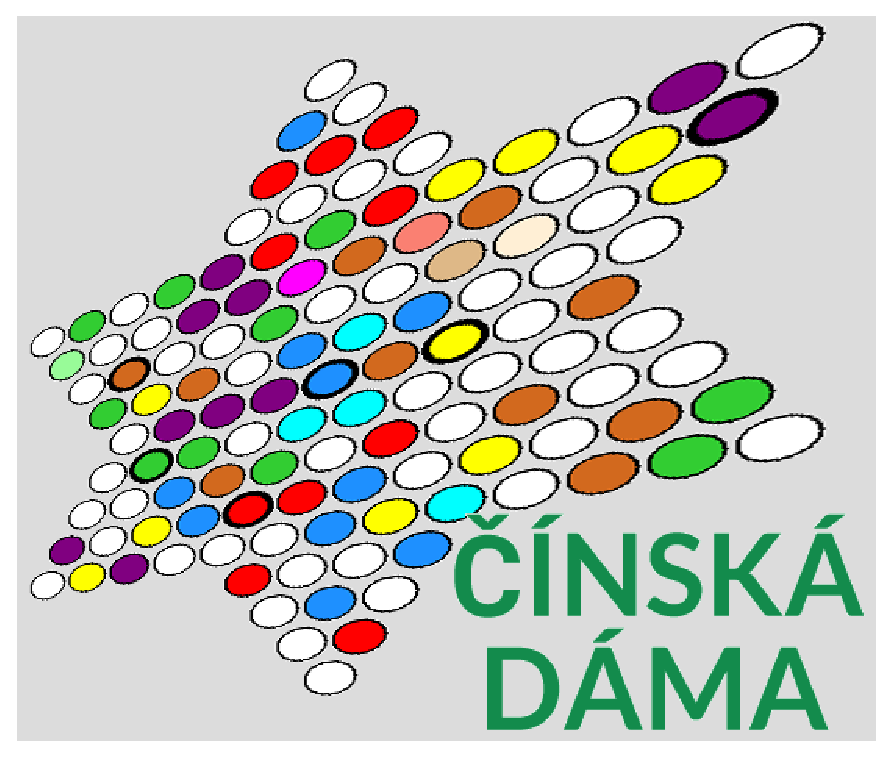
\includegraphics[scale=0.5, angle=15]{Figures/ExampleObrazek.eps}
  \caption{Obrázek vložený prostředím \texttt{graphicx}.}
  \label{obr.graphicx}
  \end{center}
\end{figure}

\begin{music}
\parindent10mm
\instrumentnumber{1}       
\setname1{Piano}           
\setstaffs1{2}             
\generalmeter{\meterfrac44}
\startextract             
\Notes\ibu0f0\qb0{cge}\tbu0\qb0g|\hl j\en
\Notes\ibu0f0\qb0{cge}\tbu0\qb0g|\ql l\sk\ql n\en
\bar
\Notes\ibu0f0\qb0{dgf}|\qlp i\en
\notes\tbu0\qb0g|\ibbl1j3\qb1j\tbl1\qb1k\en
\Notes\ibu0f0\qb0{cge}\tbu0\qb0g|\hl j\en\endextract                
\end{music}

{\fontfamily{pcr}\selectfont
Font Courier
}

{\fontfamily{lmdh}\selectfont
Font Latin Modern Dunhill
}



\endinput